\documentclass{beamer}
\usepackage[italian]{babel}
\usepackage[latin1]{inputenc}
\usepackage{amsmath}
\usepackage{amssymb}
\usepackage{latexsym}
%\usepackage{pgfplots}
\usepackage{listings}
\usepackage{graphicx}
\usepackage{etoolbox}
\usepackage{subfiles}
\AfterEndEnvironment{lstlisting}{\leavevmode}

\usepackage{tikz}
\usetikzlibrary{quotes,angles,positioning}
\usepackage{xcolor} % for setting colors
% set the default code style
\lstset{
    language=Java,
    breaklines = true,
    basicstyle=\ttfamily\scriptsize,
    tabsize=3,
    showstringspaces=false,
    numbers=none,
    keywordstyle=\color{blue},
    stringstyle=\color{red},
    commentstyle=\color{gray}
}


%\usetheme{Szeged}
%\usetheme{Darmstadt}
\usetheme{Frankfurt}
%\usetheme{AnnArbor}
%\usetheme{Berkeley}
%\usetheme{Madrid}
%\usetheme{Hannover}
%\usetheme{Luebeck}
%\usetheme{Berlin}
%\usetheme{Rochester}
%\usetheme{default}
%\usetheme{Warsaw}

%\usecolortheme{spruce}
%\usecolortheme{dolphin}
%\usecolortheme{rose}
%\usecolortheme{seahorse}
%\usecolortheme{whale}
%\setbeamertemplate{navigation symbols}{}

%------------------------------------------------------------
%This block of code defines the information to appear in the
%Title page
\title {Generazione automatica ed esecuzione di casi di test per la libreria Java JSetL}

%\subtitle{Automatic generation and execution of test cases for the Java library JSetL}

\author[Vetere F.] {
\large{\emph{Candidato:} Francesco Vetere}\texorpdfstring{\\\small{\emph{Relatore:} Prof. Gianfranco Rossi}}{}}

\institute[Universit\`a di Parma]
{
Universit\`a di Parma\\
Dipartimento di Scienze Matematiche, Fisiche e Informatiche\\
Corso di Laurea in Informatica
}

\date {26 Settembre 2019}

%End of title page configuration block
%------------------------------------------------------------

\usepackage{algorithm}
\usepackage{algpseudocode}
\renewcommand{\algorithmicrequire}{\textbf{Input:}}
\renewcommand{\algorithmicensure}{\textbf{Output:}}

\begin{document}

%The next statement creates the title page.
\begin{frame}
\maketitle
\end{frame}

%This block of code is for the table of contents after
%the title page
%\begin{frame}
%\frametitle{Sommario}
%\tableofcontents
%\end{frame}

\begin{frame}{Struttura della presentazione}
    \begin{itemize}
    \setlength\itemsep{1em}
        \item {\large Obiettivi}
        \item {\large Contesto}
            \begin{itemize}
                \item [-] Testing
                \item [-] JSetL
                \item [-] \{log\}
            \end{itemize}
        \item {\large Approccio utilizzato}
        \item {\large Lo strumento realizzato}
        \begin{itemize}
                \item [-] Architettura
                \item [-] Esempi d'uso
                \item [-] Analisi dei tempi
            \end{itemize}
        \item {\large Conclusioni e sviluppi futuri}
    \end{itemize}
\end{frame}

\section{Obiettivi}
\begin{frame}{Obiettivi}

    %\setbeamercolor{block title}{fg=blue}
   
        {
        \begin{block}{Obiettivi}
        \begin{itemize}
        \setlength\itemsep{2em}
        \item Testing sistematico ed esaustivo dei \emph{vincoli} della libreria Java JSetL.
        \item Testing affrontato dal punto di vista della soddisfacibilit\`a: per ogni vincolo, istanziato su una particolare combinazione di argomenti, si vuole ottenere un risultato (booleano) dal solver di JSetL.
		\end{itemize}        
        \end{block}
        } 

\end{frame}

\section{Contesto}
\begin{frame}{Testing}
    %\setbeamercolor{block title}{fg=blue}
   
        {
        \begin{block}{Categoria di testing}
        \begin{itemize}
        \setlength\itemsep{1em}
        \item Black-box testing\\
			\begin{itemize}        
        		\item[]Utente non obbligato a conoscere i dettagli implementativi della libreria oggetto del testing.
        	\end{itemize}        
        \item Equivalence Class Partitioning\\
			\begin{itemize}         	
       			\item[]Spazio dei possibili input suddiviso per classi di equivalenza:\\
       			test vector costruito scegliendo da ogni classe un valore campione.
       		\end{itemize}  

		\end{itemize}        
        \end{block}
        }
    %\setbeamercolor{block title}{fg=blue}
   
        {
        \begin{block}{Fase del processo di testing interessata}
        \begin{itemize}
        \setlength\itemsep{1em}
        \item Unit testing\\
        
        	\begin{itemize}  
        	\item[]Testing relativo ai moduli di base di un sistema software\\ (Framework JUnit 4).\\
        	\end{itemize}  

        \end{itemize}
        \end{block}
        }
\end{frame}

\begin{frame}{JSetL}
  		
  		%\setbeamercolor{block title}{fg=blue}
        {
        	\begin{block}{Che cos'\`e}
        	\begin{itemize}
        	\setlength\itemsep{2em}
        	\item Libreria Java che combina il paradigma O-O con il paradigma logico a vincoli.
       	 	\item JSetL implementa il linguaggio \mathcal{\emph{L}\textsubscript{\(\mathcal{SET}\)}}, linguaggio logico basato su vincoli insiemistici (nella sua successiva estensione \mathcal{\emph{L}\textsubscript{\(\mathcal{BR}\)}}, vengono trattati anche vincoli relazionali).
			\end{itemize}        
        	\end{block}	
        }

\end{frame}

\begin{frame}{Esempi di vincoli insiemistici in JSetL}

\begin{table}[]
\begin{tabular}{|l|l|l|}
\hline
\textsc{Vincolo }     & \textsc{JSetL}           & \textsc{Significato}\\ \hline
Uguaglianza  & \texttt{A.eq(B)}                 & \texttt{A} $=$ \texttt{B}                        \\ \hline
Disgiunzione & \texttt{A.disj(B)}           & \texttt{A} $\cap$ \texttt{B} $=$ $\varnothing$   \\ \hline
Unione       & \texttt{A.union(B,C)}    & \texttt{C} $=$ \texttt{A} $\cup$ \texttt{B}      \\ \hline
Intersezione & \texttt{A.inters(B,C)}  & \texttt{C} $=$ \texttt{A} $\cap$ \texttt{B}      \\ \hline
Differenza   & \texttt{A.diff(B,C)}      & \texttt{C} $=$ \texttt{A} $\setminus$ \texttt{B} \\ \hline
\end{tabular}
\end{table}

\end{frame}

%\begin{frame}{\{log\}}
    %\setbeamercolor{block title}{fg=blue}
        %{
        %\begin{block}{Che cos'\`e}
        %\begin{itemize}
        %\setlength\itemsep{2em}
        %\item Implementazione Prolog del linguaggio CLP(\(\mathcal{SET}\)) e sue relative estensioni
        %\item CLP(\(\mathcal{SET}\)) \`e il nucleo comune a JSetL e \{log\}
		%\end{itemize}        
        %\end{block}
        %}
%\end{frame}

\begin{frame}{\{log\}}
  		
  		%\setbeamercolor{block title}{fg=blue}
        {
        	\begin{block}{Che cos'\`e}
        	\begin{itemize}
        	\setlength\itemsep{2em}
        	\item Lo stesso linguaggio \mathcal{\emph{L}\textsubscript{\(\mathcal{SET}\)}} \`e implementato in ambiente Prolog attraverso \{log\}.
        	\item Il linguaggio \mathcal{\emph{L}\textsubscript{\(\mathcal{SET}\)}} \`e dunque il nucleo comune a JSetL e \{log\}.
			\end{itemize}        
        	\end{block}	
        }
        
\end{frame}

\begin{frame}{Confronto tra vincoli insiemistici in JSetL/\{log\}}

\begin{table}[]
\begin{tabular}{|l|l|l|l|}
\hline
\textsc{Vincolo }     & \textsc{JSetL}          & \textsc{\{log\}}           & \textsc{Significato}\\ \hline
Uguaglianza  & \texttt{A.eq(B)}        & \texttt{A = B}           & \texttt{A} $=$ \texttt{B}                        \\ \hline
Disgiunzione & \texttt{A.disj(B)}     & \texttt{disj(A,B)}      & \texttt{A} $\cap$ \texttt{B} $=$ $\varnothing$   \\ \hline
Unione       & \texttt{A.union(B,C)}  & \texttt{un(A,B,C)}  & \texttt{C} $=$ \texttt{A} $\cup$ \texttt{B}      \\ \hline
Intersezione & \texttt{A.inters(B,C)} & \texttt{inters(A,B,C)} & \texttt{C} $=$ \texttt{A} $\cap$ \texttt{B}      \\ \hline
Differenza   & \texttt{A.diff(B,C)}   & \texttt{diff(A,B,C)}   & \texttt{C} $=$ \texttt{A} $\setminus$ \texttt{B} \\ \hline
\end{tabular}
\end{table}


\vspace*{20px}

\begin{itemize}

\item[$\Longrightarrow$] Stesso significato, sintassi differenti\\
\end{itemize}


\end{frame}

\section{Approccio}
\begin{frame}{Approccio utilizzato}

  		%\setbeamercolor{block title}{fg=blue}
        {

        	\begin{block}{Approccio}
        	\begin{itemize}
        	\setlength\itemsep{1em}
        	\item Progettazione e sviluppo di uno strumento software \emph{ad hoc} per il testing dei vincoli della libreria JSetL.
        	\item Lo strumento software realizzato sfrutta il risolutore di \{log\} per ricavare i risultati dei singoli test, per poi riportarli su JSetL senza ricalcolarli.
			\end{itemize}        
        	\end{block}	
        }
        
         %\setbeamercolor{block title}{fg=blue}
        {
        	\begin{block}{Vantaggi}
        	\begin{itemize}
        	\setlength\itemsep{1em}
        	\item Utente non \`e costretto a conoscere in anticipo i risultati di soddisfacibilit\`a dei vincoli.
        	\item Testing indiretto di \{log\}: le due implementazioni devono mantenere coerenza.
			\end{itemize}        
        	\end{block}	
        }
\end{frame}

\section{Lo strumento realizzato}

\begin{frame}{Architettura}
	
	\begin{figure}
	\hbox{\hspace{-0.3em} 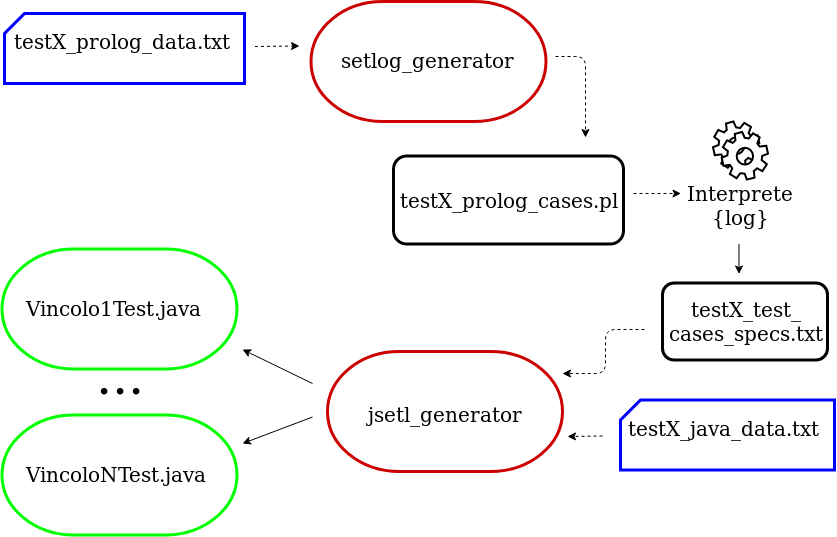
\includegraphics[scale=0.37]{architecture.png}}
	\end{figure}

\end{frame}

\begin{frame}{Esempi d'uso}
  		
  		%\setbeamercolor{block title}{fg=blue}
        {
        	\begin{block}{Collaudo dello strumento realizzato}
        	\begin{itemize}
        	\setlength\itemsep{2em}
        	\item Data la complessit\`a del processo di generazione, \`e stato inserito uno script (Linux/Windows) che esegue in automatico tutti i comandi necessari ad ogni step.
        	
        	\item Lo strumento realizzato \`e stato collaudato attraverso vari test set di prova.
        	
       	 	\item Esempio: test1
       	 		\begin{itemize}
       	 			Scopo: testing dei vincoli \texttt{eq}, \texttt{disj} e \texttt{union} su diverse tipologie di insiemi logici e loro combinazioni.
       	 		\end{itemize}
			\end{itemize}        
        	\end{block}	
        }

        
\end{frame}

\begin{frame}{Esempio: test1}
\begin{exampleblock}{test1\_prolog\_data.txt}
    \lstinputlisting[basicstyle=\ttfamily\scriptsize]{test1_prolog_data.txt}
\end{exampleblock}
\end{frame}

\begin{frame}{Esempio: test1}
\begin{exampleblock}{test1\_java\_data.txt}
    \lstinputlisting[basicstyle=\ttfamily\scriptsize]{test1_java_data.txt}
\end{exampleblock}
\end{frame}

\begin{frame}{Esempio: test1}
\begin{exampleblock}{DisjTest.java}
    \lstinputlisting[language=Java,basicstyle=\ttfamily\scriptsize]{DisjTest.java}
\end{exampleblock}

\begin{itemize}
\item Se $n$ \`e l'arit\`a di un vincolo ed $m$ sono i diversi argomenti specificati nei file di input, verranno generati $n^m$ metodi di test
\end{itemize} 
 
\end{frame}


\section{Tempi di esecuzione}


\begin{frame}{Analisi dei tempi di esecuzione}
  		
  		%\setbeamercolor{block title}{fg=blue}
        {
        	\begin{block}{ }
        	\begin{itemize}
        	\setlength\itemsep{2em}
        	\item Oltre al testing di soddisfacibilit\`a, prevista (opzionalmente) anche l'analisi dei tempi di esecuzione.
       	 	\item Utile per evidenziare in che modo i vincoli riescano a scalare all'aumentare della cardinalit\`a degli insiemi.
			\end{itemize}        
        	\end{block}	
        }

\end{frame}

\begin{frame}{test1}
	\begin{figure}
	%\hbox{\hspace{-1.0em}
	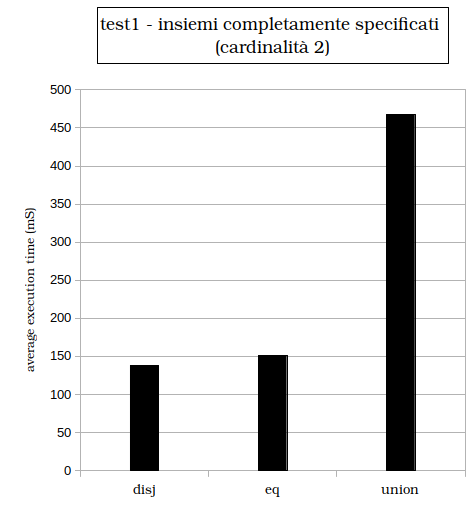
\includegraphics[scale=0.5]{histogram_test1.png}
	
	%}
	\end{figure}

\end{frame}


\begin{frame}{test11}
	\begin{figure}
	%\hbox{\hspace{-1.5em} 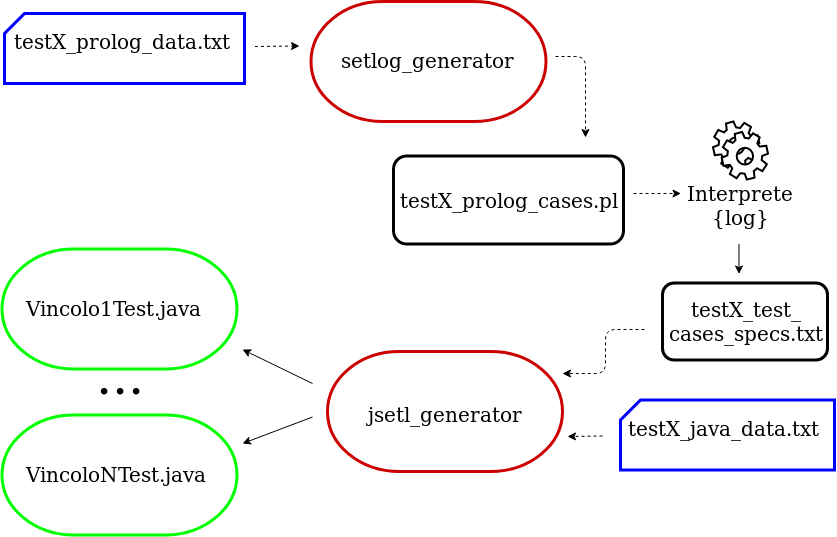
\includegraphics[scale=0.37]{architecture.png}}	

	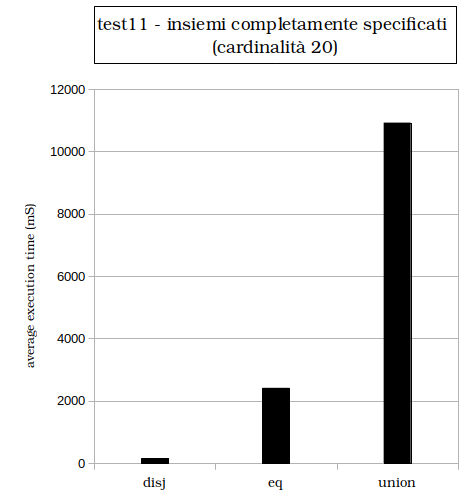
\includegraphics[scale=0.5]{histogram_test11.png}
	
	\end{figure}
\end{frame}

\section{Conclusioni}
\begin{frame}{Conclusioni}
\begin{block}{}
\begin{itemize}
\setlength\itemsep{2em}
\item In questo lavoro di tesi \`e stato affrontato il problema del testing dei vincoli di JSetL realizzando uno strumento software ad hoc avente il compito di generare test cases sistematici in maniera automatica.%\\\phantom{a}\\
\item La presenza dello strumento fornisce la possibilit\`a di testare la correttezza di qualsiasi vincolo presente nella libreria, nonch\'e di misurare le prestazioni relative alla loro risoluzione.
\end{itemize}
\end{block}
\end{frame}

\begin{frame}{Sviluppi futuri}
\begin{block}{}
        \begin{itemize}
        \setlength\itemsep{2em}
        \item Esplorare un possibile approccio parallelo attraverso l'esecuzione multi-thread dei metodi di test (JUnit 5).
        \item Per i vincoli soddisfacibili, dimostrare che le soluzioni prodotte da \{log\} siano prodotte anche da JSetL.
		\end{itemize} 
\end{block}
\end{frame}

\begin{frame}{  }
\centering \huge Grazie per l'attenzione
\end{frame}

\end{document}